% reducesymm/linresp/McICvi15.tex
% $Author: predrag $ $Date: 2015-10-14 00:30:40 -0400 (Wed, 14 Oct 2015) $

%% -------- editors/public switch ------------------
                  %%   logical setup, no need to edit %%%%%%%%%%
                  \newif\ifpaper \paperfalse \newif\ifPDF \PDFtrue  %%
                  \newif\ifblog \blogfalse                          %%
                  \newif\ifboyscout                                 %%
                  \boyscouttrue %% commented, WWW/drafts %%
%%%% Toggle between draft and public versions
% \boyscoutfalse % public, for hyperlinked pdf

%% ------------------ for arXiv submission ----------------------------
%
% Title:    Periodic Orbit Theory of Linear Response
% Authors:  Benjamin McInroe and Predrag Cvitanovic
% Comments: ? pages, ? pdf figures, uses revtex4
% Files:    McICvi15.tex sliceDefs.tex McICvi15.bbl
%           fig??.pdf fig??.pdf
%
%% ------------------ cut here ----------------------------------------



%                    PRE resubmission:
%                    arXiv submission:
%                    finished editing:
% Note: {revtex4} has been replaced by {revtex4-1} by APS
%       revert to {revtex4} if you have an old configuration
%       read also sliceDefs.tex
%                    finished writing:
%                    PRE submission:
%                    arXiv submission: =
% Predrag 2nd rewrite
%                    finished writing: Predrag
% Predrag completed rewrite
% Predrag
%%                   started writing:  Predrag
% Predrag                       2015-10-17
% Benjamin    1. draft McICvi15.tex             2015-10-17

        \ifboyscout
\documentclass[aps,pre,
                showpacs,
                twocolumn,
                %preprint,      %uncomment for double spacing
                groupedaddress,
                superscriptaddress,
                floatfix]{revtex4-1}
        \else
\documentclass[pre,aps,
                twocolumn,
                showpacs,
                superscriptaddress,
                groupedaddress,
                floatfix%,
                %hyperref
                ]{revtex4-1}
        \fi
%   REVTeX 4 Version 4.1r August 2010
%   Phys. Rev. appearance, change preprint to twocolumn.  Choose pra,
%   prb, prc, prd, pre, prl, prstab for journal Add
%   'draft' option to mark overfull boxes with black boxes Add
%   'showpacs' option to make PACS codes appear Add 'showkeys' option
%   to make keywords appear

\input setupLinresp
\ifPDF
    \bibliographystyle{apsrev4-1} %with DOI hyperlinks
\else % prepare B&W file
    \bibliographystyle{apsrev}
\fi
\input ../inputs/editsDasbuch %% editing comments, DasBuch style
\input defsLinresp %% all diffusion project edits: \renewcommand, etc

\begin{document}
\title{Periodic Orbit Theory of Linear Response}
\author{Benjamin McInroe}
\author{Predrag Cvitanovi\'c}
\email[]{predrag@gatech.edu}
\homepage[]{ChaosBook.org}
\thanks{Partially supported by NSF Grant DMS-1211827}
\affiliation{School of Physics, Georgia Institute of Technology, Atlanta  GA}

\date{\today}

\begin{abstract}
We apply periodic orbit theory to dynamical systems of
the form $\frac{d\ssp_{i}}{dt}+\epsilon \delta v_{i}(\ssp), \epsilon \ll 1$,
where $\delta v_{i}(\ssp)$ is a spatial perturbation to the flow. Such a
perturbation results in a shift of the eigenvalue spectrum of the
{\evOper} of the dynamical system, which to linear order for
structurally stable dynamics can be computed in terms of the cycle
expansion of the flow. Assuming the perturbations to the local traces
vary smoothly with the parameter $\epsilon$, the variation of the
 given observable with respect to $\epsilon$ can
also be computed. We apply this formalism to computation of the leading
eigenvalues of two one-dimensional maps, the tent map and the logistic
map, to demonstrate the results for both a structurally stable and
structurally unstable case, respectively. Finally, we apply the formalism
to computation of the Lyapunov exponent.
\end{abstract}

\maketitle



\section{Introduction}
\label{sect:intro}

In this paper we consider the dynamics of weakly perturbed systems of
the form
\(
\frac{d\ssp_{i}}{dt}=v_{i}(\ssp) + \epsilon \delta v_{i}(\ssp)
\,.
\) %ee{peturbDynSys}
The study of such systems is relevant to the statistical mechanics of
nonequilibrium systems, in which the perturbation might signify an
external force that driving the system away from a steady state. The
parameter $\epsilon$ is taken to be sufficiently small such that the
perturbing flow may be approximated to linear order. The
theory problems of this nature has come to be
called linear response theory (for a review, see Ruelle\rf{Ruelle09}).
We consider here an
approach to linear response problems based on the periodic
orbit theory\rf{DasBuch} to make predictions for expectation values of
observables.  \refSect{sect:review} is an overview of periodic orbit
theory used in developing the linear response formalism in
\refsect{sect:LinRespPO}. In \refsect{sect:tests}, the linear response
theory is applied to computations of eigenvalues for one dimensional
maps. In \refsect{sect:LyapExp} and \refsect{sect:concl}, we expand these
results to computation of the Lyapunov exponent of these maps, and
compare the results to the `classical' computation by
Abramov\rf{Abramov14}.

\section{A brief review of cycling}
\label{sect:review}

This section contains an overview of concepts from periodic orbit
theory\rf{DasBuch} used in this study.

\subsection{Zeta functions, cycle expansions, and all that}
\label{sect:ZetaFcts}

Consider a dynamical system  $(\pS,f)$ given by a measure preserving
flow, $f: \pS\rightarrow \pS$, where $\pS$ is the \statesp. If the
dynamical system is chaotic, then it is impossible to compute the
long-time trajectory for a generic initial point $\ssp_{0}\in \pS$. But all
is not lost, as we can trade the notion of a single initial point
$\ssp_{0}$ evolved forward in time by the flow $f$, for an initial
density of points, $\rho (\ssp, 0), \ssp\in \pS$, evolved forward in time by
the {\evOper} $\Lop^{t}$.
Our ultimate goal is the computation of expectation values of observables for
the dynamical system $(\pS,f)$, and thus we turn our attention to the spectrum of
the {\evOper}. Our method of choice here is by construction of
the dynamical zeta function, which has the Euler product form,
\beq
\frac{1}{\zeta} = \prod_{p} (1 - t_{p})
\eeq
where $t_{p}$ is the weight associated with the prime cycle p. The
eigenvalues of the {\evOper} are then given by the zeros of the
dynamical zeta function, that is,
\beq
{1}/{\zeta (s_{\alpha})} = 0
\ee{zetaZero}
For the $\alpha^{th}$ eigenvalue, $s_{\alpha}$. To compute the zeros,
consider the expansion of the zeta function in a formal power series,
\beq
\frac{1}{\zeta} = 1 - \sum_{p_{1}+p_{2}+\cdots+p_{k}}^{'}t_{p_{1}+p_{2}+\cdots+p_{k}}
\eeq
for $t_{p_{1}+p_{2}+\cdots+p_{k}} =
(-1)^{k+1}t_{p_{1}}t_{p_{2}}\cdots t_{p_{k}}$, where the prime on the sum
indicates that the sum is taken over all distinct, non-repeating
combinations of prime cycles. When $k>1$, $t_{p_{1}+p_{2}+\cdots+p_{k}}$ are
weights of pseudocycles, sequences of shorter cycles the shadow a cycle
with symbol sequence $p_{1}p_{2}\cdots p_{k}$, along the segments $p_{1},
p_{2}, \cdots, p_{k}$. This series representation of a dynamical zeta
function or spectral determinant is known as the cycle expansion. It is a
sum over pseudocycles, ordered by increasing cycle length and
instability.

Now comes the key step. The cycle expansion for a dynamical system with
finite grammar may be regrouped into sums of fundamental contributions,
$t_{f}$, and decreasing curvature contributions, $c_{n}$. That is,
\beq
\frac{1}{\zeta} = 1 - \sum_{f}t_{f} - \sum_{n}c_{n}
\,,
\ee{cyclExp}
where the fundamental contributions $t_{f}$ are cycles with no shorter
approximants. They are the 'building blocks' of the dynamics, from which
longer orbits may be approximately pieced together. The curvature
contributions $c_{n}$ are the longer orbits pieced together from
fundamental contributions, and their shadowing approximants. For
continuous and smooth flows, orbits of similar symbolic dynamics will
traverse the same neighborhoods, and have similar weights. The result is
that for such flows, the curvature contributions to the cycle expansion
will almost cancel. The utility of cycle expansions is now clear: by
grouping the terms, we find that the cycle expansion is dominated by the
short cycles, with long cycles giving exponentially decaying corrections.
The cycle expansion for binary symbolic dynamics is computed in
\refappe{appe:cyclBinarySymbolic}.

\subsection{Averaging for cyclists}
\label{sect:AverCycl}

We now use the formalism of the previous section to compute expectation values of
observables. Consider the weight for the cycle $p$,
\bea
t_{p} &=& t_{p}(\beta, s(\beta))
       = \frac{1}{|\ExpaEig_{p}|} e^{\beta \Obser_{p} - s(\beta)\period{p}}
\continue
       &=& \exp\left[\beta \Obser_{p} - (s(\beta)+\eigRe_p)\period{p}\right]
\,,
\label{cyclWeight}
\eea
where $\ExpaEig_{p}$ is the Floquet multiplier, $\eigRe_{p}$ the real
part of the Floquet exponent, $\Obser_{p}$ is the integrated observable
of interest, and $\period{p}$ is cycle period (or topological cycle
length for discrete dynamics). With this weight, \refeq{zetaZero} is now
an implicit equation for $s=s(\beta)$, for arbitrary parameter $\beta$,
of the form $G(\beta, s(\beta)) = 0$. The {\cycForm s} for the slope and
curvature of $s(\beta)$ follow from differentiation of the eigenvalue
condition with respect to $\beta$,
\begin{eqnarray*}
0 = \frac{d G}{d\beta}
= \frac{\pde G}{\pde \beta} + \frac{\pde s}{\pde \beta}\frac{\pde G}{\pde s}
\\
\Rightarrow \frac{\pde s}{\pde \beta} = -\frac{\pde_{\beta}G}{\pde_{s} G}
\end{eqnarray*}
Denoting by
\begin{eqnarray*}
&\expct{\Obser}_{G}& = -\frac{\pde G}{\pde \beta}|_{\beta, s=s(\beta)}
,\\ &\expct{\period{}}_{G}& = \frac{\pde G}{\pde s}\vert_{\beta, s=s(\beta)}
\,,
\end{eqnarray*}
respectively the mean cycle expectation value of $\Obser$ and the mean cycle
period, both weighted by $G$. The {\cycForm} for the
expectation value of the observable is then
\beq
\expct{\obser} = \frac{\expct{\Obser}_{G}}{\expct{\period{}}_{G}}
\ee{expectObserv}
For $G = 1/\zeta$, we obtain the zeta - weighted {\cycForm s}. Using
the cycle expansion representation,
\begin{eqnarray*}
&\expct{\Obser}_{\zeta}
  &:=-\frac{\pde}{\pde \beta}\frac{1}{\zeta}
  =\sum^{'}(\Obser_{p_{1}}+\Obser_{p_{2}}+\cdots+\Obser_{p_{k}})t_{p_{1}+p_{2}+\cdots+p_{k}} \\
&\expct{\period{}}_{\zeta}&:=\frac{\pde}{\pde s}\frac{1}{\zeta}=\sum^{'}(T_{p_{1}}+T_{p_{2}}+\cdots+T_{p_{k}})t_{p_{1}+p_{2}+\cdots+p_{k}}
\end{eqnarray*}
These are the dynamical zeta function averages over prime cycles, with
cycle weights evaluated at leading eigenvalues $t_{p} =
t_{p}(\beta,s(\beta))$. For bounded flow, $s(0)=0$, so
\begin{eqnarray*}
&\expct{\Obser}_{\zeta}& = \sum^{'}(-1)^{k+1}\frac{\Obser_{p_{1}}+\Obser_{p_{2}}+\cdots+\Obser_{p_{k}}}{\vert \ExpaEig_{p_{1}}\cdots\ExpaEig_{p_{k}}\vert}\\
&\expct{\period{}}_{\zeta}& = \sum^{'}(-1)^{k+1}\frac{T_{p_{1}}+T_{p_{2}}+\cdots+T_{p_{k}}}{\vert \ExpaEig_{p_{1}}\cdots\ExpaEig_{p_{k}}\vert}
\,.
\end{eqnarray*}
As before, these cycle expansions are grouped into fundamental and
curvature terms, with nearby pseudoorbits nearly vanishing. All zeta
weighted averages in this paper are weighted with \refeq{cyclWeight}. The
{\cycForm s} are worked out explicitly for binary symbolic
dynamics in \refappe{appe:cyclBinarySymbolic}.

\section{Linear response in terms of periodic orbits}
\label{sect:LinRespPO}

In \refsect{sect:AverCycl}, we discuss the theoretical formalism for the
periodic orbit theory approach to linear response. In
\refsect{sect:CyclAver}, we use the one dimensional unimodal tent map as
a simple, exactly solvable example of the technique, and as a prelude to
the continuous time case. In \refsect{sect:XX} we consider...

\subsection{Eigenvalue shift using dynamical zeta function}
\label{sect:EigeShiftZeta}

Consider an autonomous dynamical system of the form
\beq
\frac{d\ssp_{i}}{dt}=v_{i}(\ssp)
\,.
\ee{eqMotion}
The eigenvalues $s_{\alpha}$ of the associated {\evOper} satisfy
the dynamical zeta function condition
%\refeq{zetaZero},
\beq
{1}/{\zeta_{0} (s)} = 0
\,.
\ee{invZeta}
Under a small perturbation to the flow
% $\epsilon \delta v_{i}(\ssp)$,
the system becomes
\beq
\frac{d\ssp_{i}}{dt}=v_{i}(\ssp) + \epsilon \delta v_{i}(\ssp), \vert\epsilon\vert \ll 1
\,.
\label{pertflow}
\eeq

The result of such a perturbation is a small shift in the eigenvalues of
the {\evOper}, $s_{\alpha}\rightarrow s_{\alpha} +
\delta s_{\alpha}$. The eigenvalue condition for the dynamical zeta function
of the perturbed system is
\beq
1/\zeta(s_{\alpha}+\delta s_{\alpha}) = 0
\,.
\eeq
Expanding to linear order and solving for $\delta s_{\alpha}$ yields
\beq
\delta s_{\alpha} = -\frac{1/\zeta(s_{\alpha})}{\frac{\pde}{\pde s}1 / \zeta (s_{\alpha})}
\,.
\ee{cyclExpDeform}
The cycle expansion of $1/\zeta(s)$ is a cycle by cycle deformation of
$\frac{1}{\zeta_{0}}(s)\pm$ new / lost cycles. For structurally stable
dynamics, we can ignore the possibility of gaining or losing new cycles,
and expand the numerator of \refeq{cyclExpDeform} to linear order as,
\beq
\frac{1}{\zeta (s_{\alpha})} = \sum_{p}t_{p}(s_{\alpha}) + \sum_{p}\delta t_{p}(s_{\alpha})
\eeq
The first term is the cycle expansion of the zeta function of
\refsect{sect:ZetaFcts}, and is zero by \refeq{invZeta}. The denominator
of \refeq{cyclExpDeform} may be evaluated by noting that to leading order,
$1/\zeta(s_{\alpha}) \cong 1/\zeta_{0}(s_{\alpha})$, then from
\refsect{sect:AverCycl},
\begin{eqnarray*}
\frac{\pde}{\pde s}\frac{1}{\zeta (s_{\alpha})}
= \frac{\pde}{\pde s}\frac{1}{\zeta_{0} (s_{\alpha})}
= \sum_{p}\frac{\pde}{\pde s}t_{p}(s_{\alpha}) \\
=  \sum_{p}\period{p}t_{p}(s_{\alpha})
=  \expct{\period{p}}_{\zeta}
\end{eqnarray*}
The numerator may be evaluated by expanding $\delta t_{p}$ in terms of
variations of $\Obser_{p}$, $\period{p}$, and $\ExpaEig_{p}$. Substituting for
\refeq{cyclExpDeform}, we find
\beq
\delta s_{\alpha}
=
-\frac{\beta \expct{\delta \Obser_{p}}_\zeta - s\expct{\delta \period{p}}_{\zeta}
- \expct{\frac{\delta \ExpaEig_{p}}{\ExpaEig_{p}}}_{\zeta}}
  {\expct{\period{}}_{\zeta}\vert_{s=s_{\alpha}}}
\,,
\ee{pertEigShift}
which is the expression for the shift of the perturbed eigenvalues.

\subsection{{\CycForm s} for linear response of observables}
\label{sect:CyclAver}

We have found that for structurally stable, hyperbolic dynamics, the
eigenvalue $s_{\alpha}$ and the characteristics of the orbits depend on
the variation parameter of the system, $\epsilon$. However, for each
fixed value of $\epsilon$, the {\cycForm} should be
applicable, thus
\begin{eqnarray}
\frac{\pde \expct{a}_{\zeta}}{\pde \epsilon}
= \frac{\pde}{\pde \epsilon}\frac{\expct{A}_{\zeta}}{\expct{\period{}}_{\zeta}}
= \frac{\frac{\pde \expct{A}_{\zeta}}{\pde \epsilon}
   - \expct{a}_{\zeta}
   \frac{\pde \expct{\period{}}_{\zeta}}
        {\pde \epsilon}}
     {\expct{\period{}}_{\zeta}}
\,,
\label{varObserv}
\end{eqnarray}
where we have simplified the final expression with \refeq{expectObserv}.

In a typical calculation of a physical average, $\beta$ is put to zero.
For a bounded system the leading eigenvalue $s_{0}=0$ is independent of
the perturbation. In \refappe{sect:VarObsEps}, we evaluate
\refeq{varObserv} step-by-step. The result is,
\begin{eqnarray*}
&\frac{\pde \expct{a}_{\zeta}}{\pde \epsilon}
& = \frac{1}{\expct{\period{}}_{\zeta}}
        \Bigg(
    \expct{(\beta(A-\expct{a} T + 1)\frac{\pde A}{\pde \epsilon}} \\
&-& \expct{(s_{\alpha}-(1-s_{\alpha})\expct{a})\frac{\pde T}{\pde \epsilon}}  \\
&-& \expct{(A-\expct{a} T) \frac{\frac{\pde \ExpaEig}{\pde \epsilon}}{\ExpaEig}}
        \Bigg)
\end{eqnarray*}

To first order, the asymptotic average value of the observable $a(x)$ is then,

\begin{eqnarray*}
& \expct{a}_{\zeta} = \expct{a}_{\zeta} \bigg\rvert_{\epsilon = 0} + \frac{\pde \expct{a}_{\zeta}}{\pde \epsilon} \bigg\rvert_{\epsilon = 0} \epsilon + o(\epsilon^{2})
\end{eqnarray*}

Computation of the expectation value of an observable to first order for the perturbed dynamical system \refeq{pertflow} is thus reduced to computation of the first order partials of $A_{p}$, $T_{p}$, and $\Lambda_{p}$ in epsilon. 

    \BM{2017-02-07}{ Here is what has concerned me the past few days. Computation of $\frac{\pde \Lambda}{\pde \epsilon}$ is trivial for hyperbolic flows. But how to compute $\frac{\pde T}{\pde \epsilon}$ and $\frac{\pde A}{\pde \epsilon}$ in the general case (ie anything more challenging than the 1D unimodal repeller considered in the current draft) is not clear to me. Am I missing something obvious? }

This completes the analysis of periodic orbit theory of linear response.


\section{Results of analytic and numerical tests}
\label{sect:tests}

\subsection{Tent map}
\label{sect:tentMap}

As a simple, one dimensional discrete example to provide insight into the
application of the formalism established in the previous section, we
consider the tent map of the form
\beq
f(x) = \left\{
     \begin{array}{lr}
       \ExpaEig_{0} x & : x \in \pS_{0}\\
       \ExpaEig_{1} (1-x) & : x \in \pS_{1}
     \end{array}
   \right.
\,,
\eeq
where the two \statesp\ regions, $\pS_{0}$ and $\pS_{1}$, are partitioned by
the critical point at which the two sides of the map are equal. This type
of unimodal map is particularly desirable, as its {\evOper} has
a simple, finite dimensional form\rf{Driebe99}. As a result, the leading
eigenvalue $s_{0}$ may be written analytically as
\beq
s_{0} =
\ln\left( \frac{1}{|\ExpaEig_{0}|}+\frac{1}{|\ExpaEig_{0}|}\right)
\ee{leadEig}
where $|\ExpaEig_{i}|$ are the slopes of the left and right sides
of the map, see \reffig{fig:tentmapexample}.

\begin{figure}[htbp]
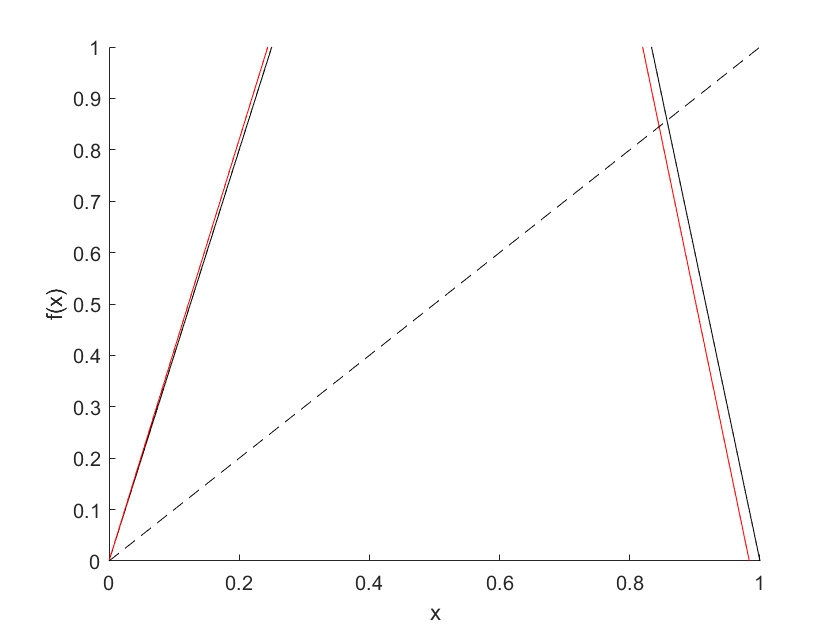
\includegraphics[width=0.45\textwidth]{tentmapexample}
\caption{\label{fig:tentmapexample}
The tent map repeller \refeq{eq:tentmapexample}. (black lines)
The unperturbed tent map with $|\ExpaEig_{0}|=4$,
$|\ExpaEig_{1}|=6$. (red lines) A perturbed tent
map, with perturbation  $\epsilon=0.1$.
        }
\end{figure}
Consider a perturbation to the tent map that slightly shifts the slopes
of the two sides. That is, a perturbation of the form,
\beq
f(x) = \left\{
     \begin{array}{lr}
       \ExpaEig_{0} x+\epsilon x & : x \in \pS_{0}\\
       \ExpaEig_{1} (1-x)-\epsilon x & : x \in \pS_{1}
     \end{array}
   \right.
\ee{eq:tentmapexample}
for $|\epsilon |\ll 1$. The example for $\epsilon=
0.1$ is plotted in \reffig{fig:tentmapexample}.

    \PC{2017-01-15}{ Is $\epsilon= 0.1$ really what is plotted in
    \reffig{fig:tentmapexample}? }
    \BM{2017-02-08}{ Good point - it certainly doesn't look like it. Fixed :) }
    
The perturbation is
conveniently chosen such that it shifts the values of the Floquet
multipliers by $+\epsilon$, and the leading eigenvalue can be computed
exactly from \refeq{leadEig}. Using the periodic orbit theory approach from
\refsect{sect:EigeShiftZeta}, the approximate shift of the leading
eigenvalue can be computed from \refeq{pertEigShift}. Taking $\beta=0$,
and noting that for the example in \reffig{fig:tentmapexample}, with
$\epsilon\in [0,1]$, the perturbation does not change the symbolic
dynamics, so that the second term in the numerator also vanishes,
\beq
\delta s_{\alpha}
  = \frac{1}{\expct{\period{}}_{\zeta}}
    \expct{\frac{\delta \ExpaEig_{p}}{\ExpaEig_{p}}}_{\zeta}
\,.
\eeq
The computation is straightforward for binary symbolic dynamics, and may
be found in \refappe{appe:cyclBinarySymbolic}. A comparison of the exact
and linear response results is plotted in \reffig{fig:numeric}. In
particular, curvature terms are neglected when evaluating the {\cycForm
s} used in \reffig{fig:numeric} in order to simplify computations.

\begin{figure}[htbp]
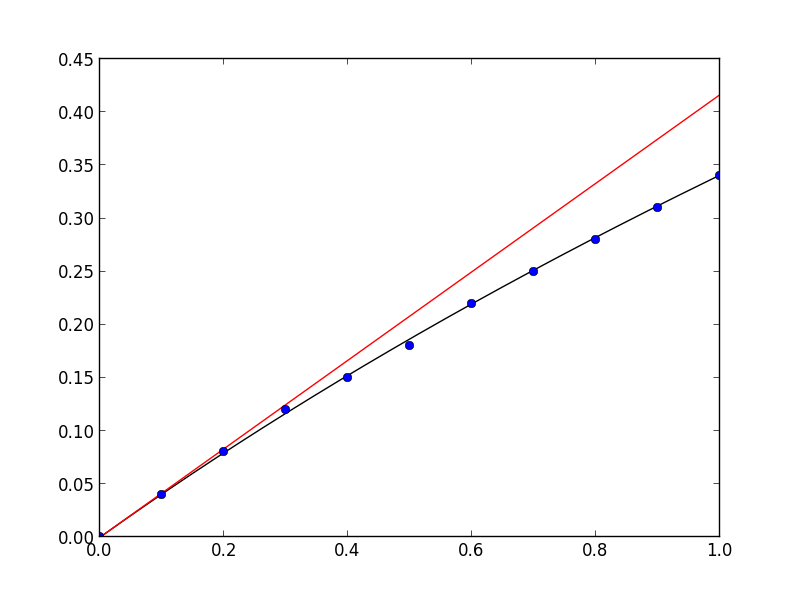
\includegraphics[width=0.45\textwidth]{numeric}
    \caption{\label{fig:numeric}
Results of the tent map repeller exact (black), linear response (red),
and numerical (blue points) calculations of eigenvalue shift for the map
in \reffig{fig:tentmapexample}.
% For $\epsilon$ sufficiently small, the results agree to high precision.
The numerical calculation is done for
the physical interpretation of the leading eigenvalue as the escape rate
of the repeller, $\gamma = -s_{0}$.
    }
\end{figure}

\subsection{Logistic map}
\label{sect:logstMap}

In \refsect{sect:LinRespPO}, we made the assumption that the dynamics of the
perturbed system are structurally stable, that is, the perturbing flow
does not create or destroy fixed points or periodic orbits. What if we
were to choose a case for which this is not true? Would the linear
response theory still provide a good approximation for the eigenvalue
shift? To help answer these questions, we start by considering one of the
simplest nonlinear maps with chaotic properties, the logistic map\
\beq
f(x) = rx(1 - x), x\in [0, 1]
\,,
\ee{logstMap}
for which a small perturbation to the parameter r can result in a period
doubling bifurcation. We consider a parameter perturbation of the form
$r \to r+\epsilon$,
\beq
\epsilon \delta f(x) = \epsilon x(1-x), |\epsilon|\ll 1
\eeq
The symbolic dynamics are again binary, so computation of the actual
eigenvalues is done as in the previous section.

\begin{figure}[htbp]
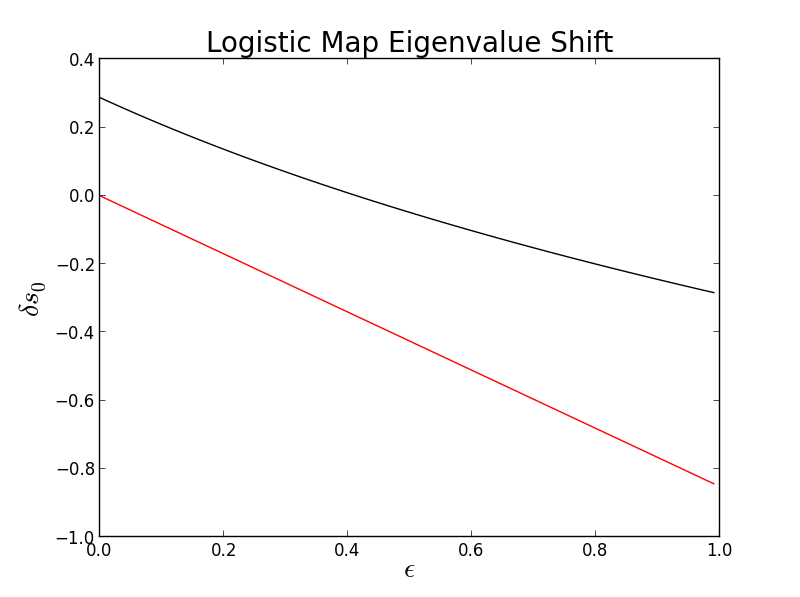
\includegraphics[width=0.45\textwidth]{logisticnumeric}
    \caption{\label{fig:logisticnumeric}
Results of the logistic map exact (black), linear response (red), and
numerical (blue points) calculations of eigenvalue shift for logistic map
\refeq{logstMap}, with unperturbed $r=3.0$. There is no value of
$\epsilon$ for which the linear approximation is close to the actual
eigenvalue shift.
        }
\end{figure}

\section{Calculation of Lyapunov exponent}
\label{sect:LyapExp}

We now turn our attention to the calculation of a 'real' observable for
the perturbed maps, the Lyapunov exponent. The Lyapunov exponent is
sometimes considered to be an indicator of a chaotic dynamical system,
with chaotic dynamics having a positive Lyapunov exponent, corresponding
to exponential divergence of flows for nearby initial conditions.

\subsection{Derivation of Lyapunov exponent}

Let $\bf x(t)$ be an orbit of the set of differential equations (7) with
initial state $\bf \ssp_{0}$, that is, $\textbf{x(t)} = f^{t}(\textbf{$\bf
\ssp_0$})$, where $f^t$ is the flow of (7). For a small perturbation to this
initial state, $\bf \delta \ssp_{0}$, we have another orbit, $\textbf{x(t)}
+ \textbf{$\bf \delta x(t)$}$ = $f^{t}(\textbf{$\bf \ssp_{0}$} +
\textbf{$\bf \delta \ssp_{0}$})$. As our ansatz, suppose that as the orbits
evolve, the separation $\bf \delta \ssp_{0}$ grows as,

\beq
e^{\lambda t} \approx \left\Vert \frac{\bf \delta x(t)}{\bf \delta \ssp_{0}} \right\Vert
\eeq

Rearranging, this expression becomes exact in the limit,

\beq
\lambda = \lim_{t\rightarrow \infty} \frac{1}{t} \sum_{i} t_{i} \lambda_{i}
\eeq
Where $t = \sum_{i} t_{i}$. In practice, one would let the separation
grow until $\Vert \bf \delta x(t_{1}) \Vert$ is sufficiently large (at
time $t_{i}$), record the value of the Lyapunov exponent, re-scale back
to the linear regime, and continue ad infinitum.

If we let the initial separation tend to zero, then,
\beq
\lim_{\bf \delta \ssp_{0} \rightarrow 0} \frac{\bf \delta x(t)}{\bf \delta \ssp_{0}}
= \frac{\bf \pde x(t)}{\bf \pde \ssp_{0}}
= J^{t}(\bf \ssp_{0})
\,,
\eeq
where $J^{t}$ is the Jacobian matrix of the flow at time $t$. It follows
then that the leading Lyapunov exponent is
\beq
\lambda(\textbf{$\ssp_{0}$})
= \lim_{t\rightarrow \infty}\frac{1}{t}
\ln \frac{\Vert J^{t}(\textbf{$\ssp_{0}$}) \textbf{$\delta \ssp_{0}$} \Vert}
         {\Vert \textbf{$\delta \ssp_{0}$} \Vert}
\,.
\eeq

\subsection{Lyapunov exponent }

\subsection{Linear response for Lyapunov exponent - classical formulation}
\label{sect:LinrespLyapClass}

\subsection{Linear response for Lyapunov exponent - cyclist's formulation}
\label{sect:LinrespLyapCycl}

\section{Summary and conclusions}
\label{sect:concl}

We have developed here the periodic orbit formalism for the computation of the
linear response of eigenvalues for a general, $d$-dimensional system of
differential equations. Furthermore, we applied our result to the
calculation of the shift in the eigenvalue spectrum of one dimensional
maps with both a hyperbolic and non-hyperbolic fixed point. As expected,
while the periodic orbit theory result for the shift in the eigenvalue
spectrum was valid for small perturbations in the hyperbolic case, the
approximation broke down in the non-hyperbolic case, yielding incorrect
results for even the zero perturbation case. Specifically, there is no
reason to assume that cycle-expansion parameters vary continuously with
respect to the perturbation parameter in the non hyperbolic case,
rendering the formalism we developed in \refsect{sect:LinRespPO} useless for such cases.

In Sec. V, we showed the utility of the periodic orbit approach for
calculating the linear response of the Lyapunov exponent of the one
dimensional maps from before. We recover the result from Abramov's
calculation, but exchange integrals over long trajectories for finite
sums over a few prime cycles.

A natural extension of this work would be to compute observables for a
higher dimensional system, in which case the utility of the periodic
orbit approach will be even more obvious.

We find that while the linear response theory can provide a reasonable
approximation to the shift in spectrum brought on by a small
perturbations for hyperbolic, structurally stable dynamics, the
approximation fails for flows without these properties, even in the case
of simple one dimensional maps. Although the linear perturbation approach
seems like a natural solution for analyzing dynamical systems subject to
small perturbations, it is complicated by the high sensitivity to
parameters and potential for bifur- cations present in chaotic systems.
In particular, there is no reason to assume that cycle expectation values
vary continuously with the perturbation parameter as we assumed in
\refsect{sect:LinRespPO}, rendering our equations for spectrum variation
nearly useless, as in \reffig{fig:logisticnumeric}.
While the tent and logistic map examples provide a taste of how the
spectra of evolution operators respond to linear perturbations, some
interesting examples had to be left out of this draft. In particular, the
dike map\rf{dasBuch}, a tent map with a slice taken of the top, provides
an example of structurally unstable dynamics similar to the logistic map.
The possibility of symmetry breaking perturbations is particularly
interesting, and although attempts at computing linear response for
continuous flows are a work in progress at the time of this writing,
discrete maps provide perhaps a more tractable take on this problem.
Study of the Gallavotti- Cohen theorem\rf{??} for non-equilibrium systems
with periodic orbit theory might also be an interesting avenue of future
work.


\begin{acknowledgments}
This report is a continuation of a project started by S{\o}ndergaard and
Cvitanovi\'c in 1995.
We are grateful to ... for many fruitful discussions in
the early stages of this project, and ...
BM was supported by NSF grant ???-?????.
PC thanks to the family of late G. Robinson, Jr. for partial support.
\end{acknowledgments}

% Specify following sections are appendices. Use \appendix* if there
% only one appendix.
\appendix

\section{Cycle expansion for binary symbolic dynamics}
\label{appe:cyclBinarySymbolic}

The simplest example of the cycle expansion is that for the binary
symbolic dynamics, of interest when the \statesp\ $\pS$ may be partitioned
into two regions, labeled $\pS_{0}$ and $\pS_{1}$. The Euler product
representation of the dynamical zeta function is then,
\begin{eqnarray*}
\frac{1}{\zeta} &=& (1 - t_{0})(1-t_{1})(1-t_{01})(1-t_{001})(1-t_{011})
\\ &(1-t_{0001})&(1-t_{0011})(1-t_{0111})\cdots
\end{eqnarray*}
for cycles up to topological length four. Expanding the product, we
obtain the cycle expansion form of the zeta function,
\begin{eqnarray*}
\frac{1}{\zeta}
&=& 1 - t_{0} - t_{1} - t_{001} - t_{011} - t_{0001} - t_{0011} - t_{0111} - \cdots
\\
&-& t_{0+1} - t_{01+1} - t_{0+001} - t_{0+011} - \cdots
\end{eqnarray*}
Next, we regroup the terms in the above expansion into fundamental and
curvature contributions. In this example, there are only two fundamental
contributions to the cycle expansion, corresponding to the $\pS_{0}$ and
$\pS_{1}$ fixed points,
\begin{eqnarray*}
\frac{1}{\zeta} &=& 1 - t_{0} - t_{1} \\
&-& [(t_{01} - t_{1}t_{0})] \\
&-& [(t_{001} - t_{01}t_{0}) + (t_{011} - t_{01}t_{1})] - \cdots
\end{eqnarray*}
As expected, the curvature terms nearly cancel, leaving the fundamental
contributions as the dominant terms in the series, a result used to
simplify computations of {\cycForm s} in \refsect{sect:tests}. For example,
for the average cycle period, the cycle expansion with the usual weight
is,
\begin{eqnarray*}
\expct{\period{}}_{\zeta}
&=& \frac{T_{0}}{\ExpaEig_{0}} + \frac{T_{1}}{\ExpaEig_{1}}
+   \left( \frac{T_{01}}{\ExpaEig_{01}}-\frac{T_{0} + T_{1}}{\ExpaEig_{0}\ExpaEig_{1}}\right)
\\
&+& \left( \frac{T_{001}}{\ExpaEig_{001}}-\frac{T_{01} + T_{0}}{\ExpaEig_{01}\ExpaEig_{0}}\right)
+\dots
\end{eqnarray*}
This is the {\cycForm} calculated in \refsect{sect:AverCycl}
for symbolic dynamics. A similar result is found for the {\cycForm} for $\Obser$.

\subsection{Variation of $\expct{\obser}_{\zeta}$ in $\epsilon$}
\label{sect:VarObsEps}

Here we derive final equation in \refsect{sect:CyclAver} for the
variation of $\expct{a}_{\zeta}$ in the parameter $\epsilon$.
We
start by computing the variations of the cycle expectation value of $\Obser$,
\begin{eqnarray*}
\frac{\pde \expct{\Obser}_{\zeta}}{\pde \epsilon}
= \frac{\pde}{\pde \epsilon}\sum_{p}t_{p}\Obser_{p}
= \sum_{p}\left(\frac{\pde t_{p}}{\pde \epsilon}\Obser_{p}
                + t_{p} \frac{\pde \Obser_{p}}{\pde \epsilon} \right)
\end{eqnarray*}

\[
\frac{\pde t_{p}}{\pde \epsilon}
    =
\left(
  \beta \frac{\pde \Obser_{p}}{\pde \epsilon}
 -(s+\eigRe_p)\frac{\pde \period{p}}{\pde \epsilon}
 - \period{p}\frac{\pde \eigRe_p}{\pde \epsilon}
\right) t_{p}
\]

\begin{eqnarray*}
\frac{\pde \expct{\Obser}_{\zeta}}{\pde \epsilon}
= \frac{\pde}{\pde \epsilon}\sum_{p}t_{p}\Obser_{p}
= \sum_{p}\frac{\pde t_{p}}{\pde \epsilon}\Obser_{p} + \sum_{p} \frac{\pde \Obser_{p}}{\pde \epsilon} t_{p}
\\ = \sum_{p}t_{p}\Bigg( \Bigg( -s\frac{\pde \period{p}}{\pde \epsilon} + \beta \frac{\pde \Obser_{p}}{\pde \epsilon} - \frac{\frac{\pde \ExpaEig_{p}}{\pde \epsilon}}{\ExpaEig_{p}}\Bigg) \Obser_{p} +\frac{\pde \Obser_{p}}{\pde \epsilon} \Bigg)
\end{eqnarray*}


The variation of the cycle expectation value of $\period{}$ is computed the same way,
\begin{eqnarray*}
\frac{\pde \expct{\period{}}_{\zeta}}
     {\pde \epsilon}
= \frac{\pde}{\pde \epsilon}\sum_{p}t_{p}\period{p}
=   \sum_{p}\frac{\pde t_{p}}{\pde \epsilon}\period{p}
  + \sum_{p}\frac{\pde \period{p}}{\pde \epsilon} t_{p}
\\
= \sum_{p}t_{p}
      \Bigg(
          \Bigg(
-s\frac{\pde \period{p}}{\pde \epsilon}
+ \beta \frac{\pde \Obser_{p}}{\pde \epsilon}
- \frac{\frac{\pde \ExpaEig_{p}}{\pde \epsilon}}{\ExpaEig_{p}}
          \Bigg) \Obser_{p}
+\frac{\pde \period{p}}{\pde \epsilon}
      \Bigg)
\end{eqnarray*}
Substituting back into \refeq{varObserv}, we get
\begin{eqnarray*}
\frac{\pde \expct{a}_{\zeta}}{\pde \epsilon}
&=&\\
\frac{1}{\expct{\period{}}_{\zeta}}
    \Bigg(&\sum_{p}&
    t_{p}\Bigg(
            \Bigg(
-s\frac{\pde \period{p}}{\pde \epsilon}
+ \beta \frac{\pde \Obser_{p}}{\pde \epsilon}
- \frac{\frac{\pde \ExpaEig_{p}}{\pde \epsilon}}{\ExpaEig_{p}}
            \Bigg) \Obser_{p} +\frac{\pde \Obser_{p}}{\pde \epsilon}
        \Bigg)\\
- \expct{a}_{\zeta} &\sum_{p}&t_{p}
        \Bigg(
            \Bigg(
-s\frac{\pde \period{p}}{\pde \epsilon}
+ \beta \frac{\pde \Obser_{p}}{\pde \epsilon}
- \frac{\frac{\pde \ExpaEig_{p}}{\pde \epsilon}}{\ExpaEig_{p}}
            \Bigg) \Obser_{p} +\frac{\pde \period{p}}{\pde \epsilon}
        \Bigg)
    \Bigg)
\,.
\end{eqnarray*}
Regrouping terms with the same partials, and re-writing the
sums  over cycles as cycle average values, we obtain,
\begin{eqnarray*}
&\frac{\pde \expct{\obser}_{\zeta}}{\pde \epsilon}
& = \frac{1}{\expct{\period{}}_{\zeta}}
    \Bigg(
\expct{(\beta(\Obser-\expct{\obser} T + 1)\frac{\pde \Obser}{\pde \epsilon}} \\
&-& \expct{(s_{\alpha}-(1-s_{\alpha})\expct{a})\frac{\pde T}{\pde \epsilon}}  \\
&-& \expct{(\Obser-\expct{\obser} T) \frac{\frac{\pde \ExpaEig}{\pde \epsilon}}{\ExpaEig}}
    \Bigg)
\end{eqnarray*}

\bibliographystyle{apsrev4-1}
\bibliography{../bibtex/siminos,../bibtex/linresp}

%%%%%%%%%%%%%%%%%%%%%%%%%%%%%%%%%%%%%%%%%%%%%%%%
\ifboyscout
\newpage
    \section{McICvi15 flotsam}
    \label{s:flotsam}
    \input flotsam
\newpage
\fi

\end{document}
